\section{Evaluation of PREF for traffic splitting}

An individual evaluation of PREF, the splitting mechanism of PREFLEX, is required to understand better the global performance of PREFLEX. Indeed, the two components PREF and LEX are functionally separate. Hence, in this section PREF will be disassociated from the rest of the architecture and put in two other contexts. A simplified load balancer, referred to in this text as “equalization mode”, that balances the traffic in a fixed and equal fraction over all the available paths. The second scenario is in a simplified version of TEXCP that doesn't include the core routers based traffic shaping for congestion management. 

For both modes, we are going to use the topology ..,. The variation of the number pf flows in the system is kept simple with the same number of flows for both servers. Only one change was introduced to see how fast the reaction of the algorithm is. It concerns the number of flows for each destination.

\subsection{Equalization Mode}

In this mode each balancer defines an equal split over the three paths for each of the destination. Figure \ref{fig:fwnd} gives an example

 \begin{figure}[h]
  \begin{center}
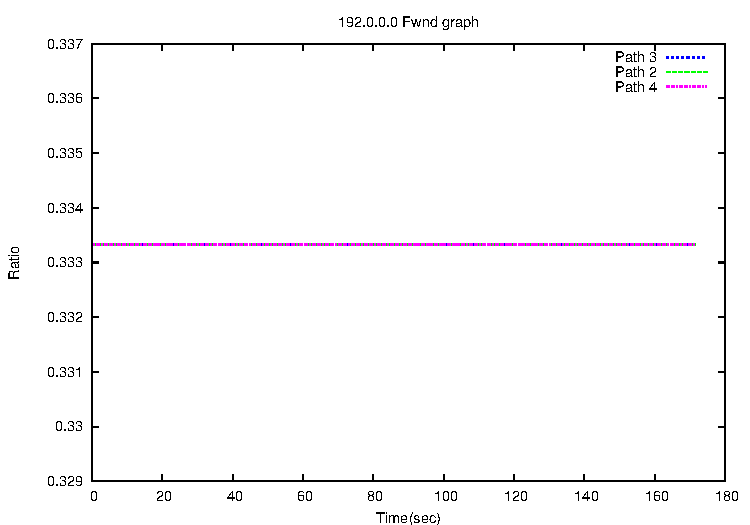
\epsfig{file=img/results/fwnd-192-0-0-0, width=4.5in}
\caption{
  Flowlet ratio $f_{i}$ for destination $E_{1}$ as set by ingress point $I_{1}$.
    \label{fig:fwnd}
}
 \end{center}
\end{figure}

The graphs bellow show the throughput of the traffic that ingress node I1 send over each link.\\

PREF

\begin{figure}[h]
 \begin{center}

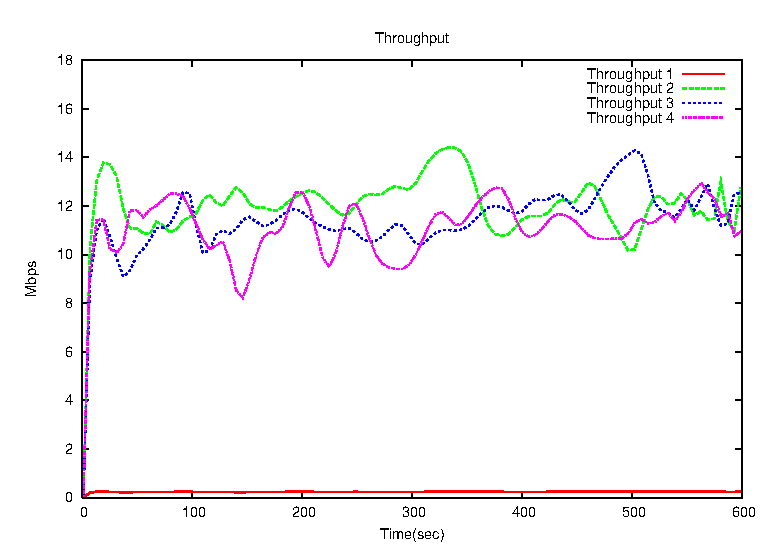
\epsfig{file=img/results/sec5-1/equalization-PREF/eleven/throuputs, width=4.5in}
\caption{
  Throughputs over each interface.
    \label{fig:equal-thro-pref}
}
\end{center}

FLARE

\end{figure}

 \begin{figure}[h!]
 \begin{center}
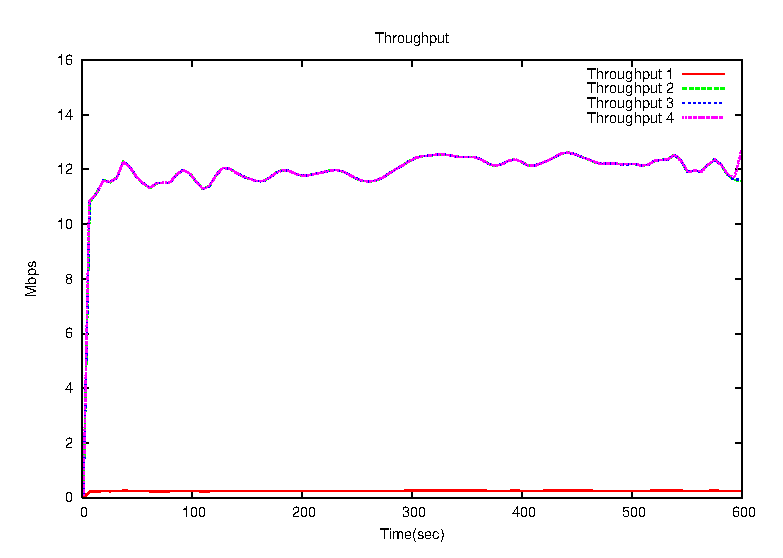
\epsfig{file=img/results/sec5-1/equalization-FLARE/eleven/throuputs, width=4.5in}
\caption{
  Throughputs over each interface.
    \label{fig:equal-thro-flare}
}
\end{center}

\end{figure}

%\begin{figure}[h]
%  \begin{center}
%    \mbox{
%      \subfigure[]{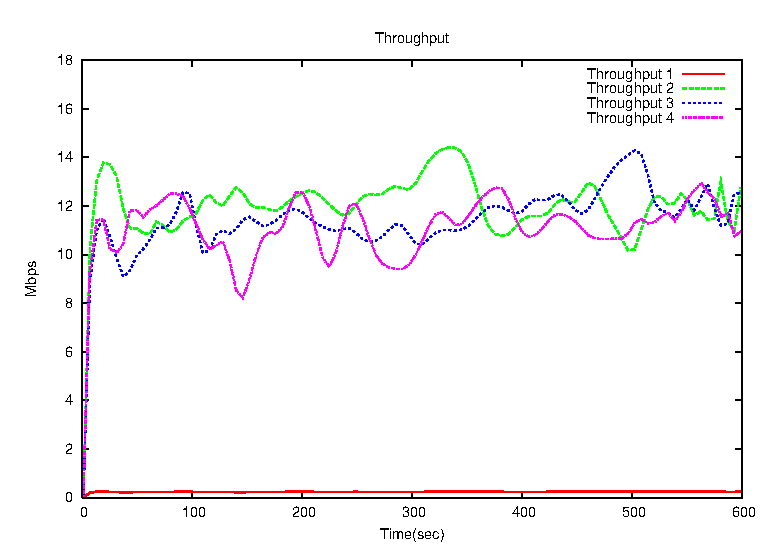
\includegraphics[width=4.0in]{img/results/sec5-1/equalization-PREF/eleven/throuputs}}\\
%      \subfigure[]{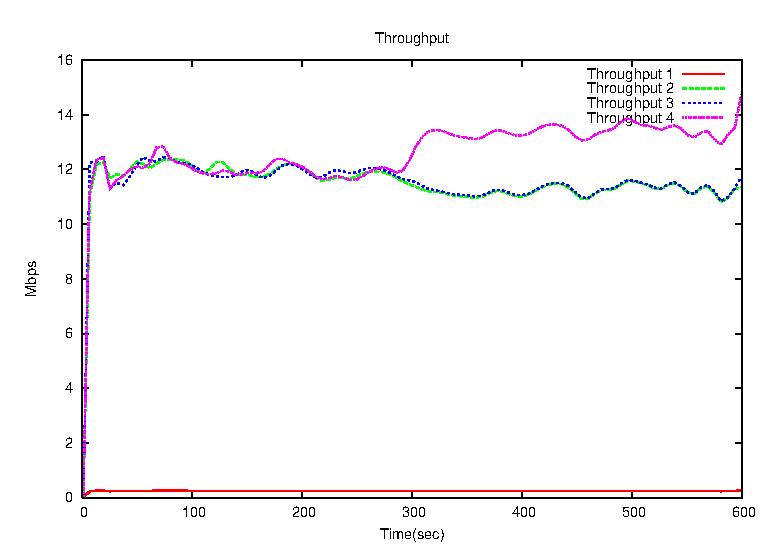
\includegraphics[width=4.0in]{file=img/results/sec5-1/equalization-FLARE/eleven/throuputs}}
%    }
%\caption{caption goes here.}
%\label{fig:parts}
%\end{center}
%\end{figure}

As expected, PREF which is equilibrium a flow based traffic splitter, doesn't match the accuracy level of FLARE in splitting the traffic, but still the difference on the throughput over each path stays limited. The graphs also show oscillation behavior of PREF. We find the same oscillation behavior in the graphs of drop rate at the bottlenecks.

PREF

\begin{figure}[h]
 \begin{center}

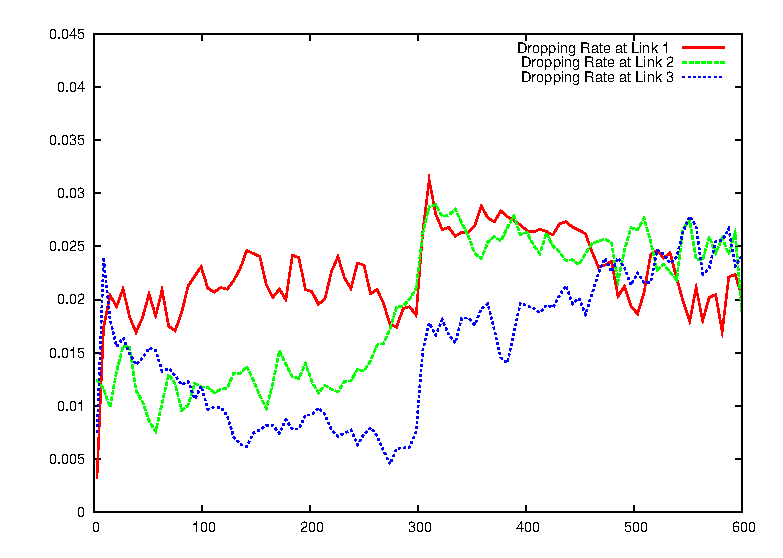
\epsfig{file=img/results/sec5-1/equalization-PREF/dropRate, width=4.5in}
\caption{
  Drop Rate at the botlenecks.
    \label{fig:equal-thro-pref}
}
\end{center}
\end{figure}

FLARE
 \begin{figure}[h!]
 \begin{center}
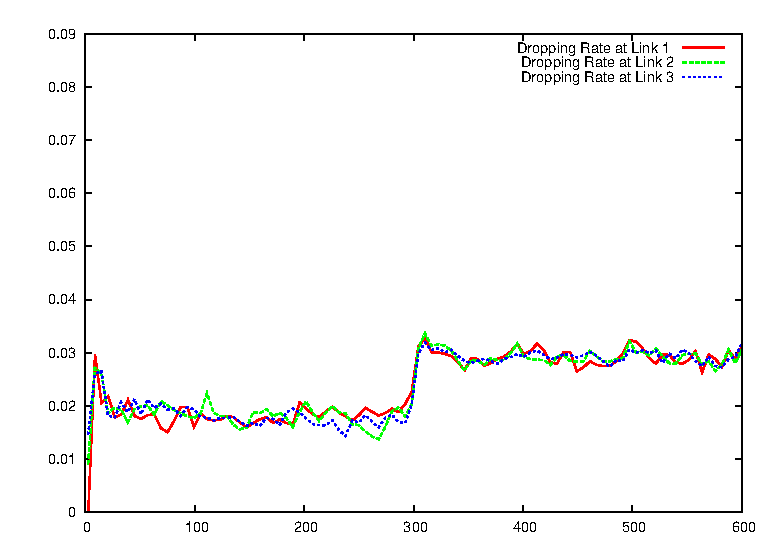
\epsfig{file=img/results/sec5-1/equalization-FLARE/dropRate, width=4.5in}
\caption{
  Drop Rate at the botlenecks.
    \label{fig:equal-thro-flare}
}
\end{center}
\end{figure}

These seconds graphs provide a hint about the reason of the fluctuation. The path assignment process of PREF makes the flowlets, which are transport aware, evolve their whole life cycle in one path and hence have a different congestion experience than the other flows. As a result, their transmission rates and the congestion they make are decorrelated. In the other hand, the network flowlets used by FLARE are a smaller order of granuilarity and makes that the transport flows get a path attributed multiple times during their flow time. As a result, the congestion level that a TCP routine experienced is a combination of the congestion in the different paths and hence the flows adapt their transmission rate to a common level of congestion and the fluctuations are less significant.

%\clearpage

\subsection{balancing by path utilization}

Now we consider the example of balancing by path utilization, a simplified version of TEXCP where ingress points don't use the core routers feedback to control their transmissions rate.

PREF

\begin{figure}[h]
 \begin{center}

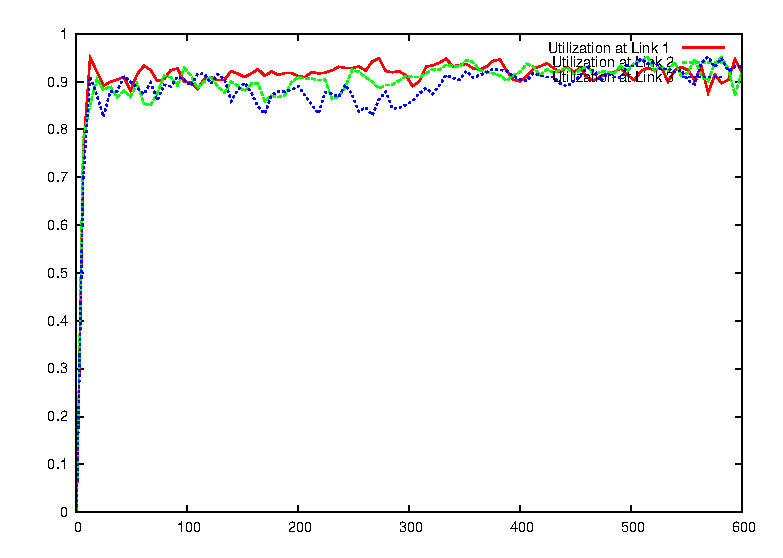
\epsfig{file=img/results/sec5-1/equalization-PREF/util, width=4.5in}
\caption{
  Path utilization measured at bottlenecks. 
    \label{fig:texcp-util-pref}
}
\end{center}
\end{figure}

FLARE
 \begin{figure}[h!]
 \begin{center}
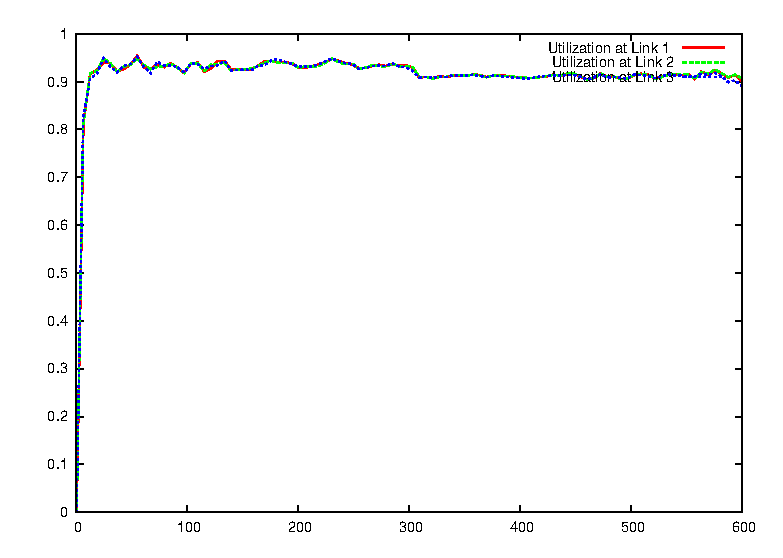
\epsfig{file=img/results/sec5-1/texcp-flare/util, width=4.5in}
\caption{
  Path utilization measured at bottlenecks. 
    \label{fig:texcp-util-flare}
}
\end{center}
\end{figure}

The previous analysis is stil valid ine the case of balamcing by path utilization. This last parameter oscillates in the case of PREF splitting, and equalization is not achieved with the same accuracy.

\paragraph{Conclusion}

Splitting traffic using PREF is required for the congestion mechanism defined by LEX. The revelation of a path congestion requires that the retransmitted packets follow the same path. Moreover, it makes congestion balancing a bit more difficult since the flows follow one path with decorelated congestion experiences. However, PREF allows path diversity schemes at end hosts and network to coexist. The performance of PREF could be enhanced further, if efficient strategies of how and when to trigger path selection were deployed at by the recievers.
 
%\section{Load balancing VS congestion balancing}
\section{Analysis of PREFLEX balancing algorithm}

In this section we are going to evaluate the performance of the algorithm for different configuration parameters. 

\subsection{Decision time interval}

The decision time interval is an external parameter for the algorithm. It determines how often the network domain updates the split. The stability of the algorithm and how long it takes to reach equilibrium is linked to the decision interval. But from another hand, this decision interval is also dependant of the period over which the loss signals are aggregated. As a result, a frequent update of the split may result in an instability of the system that will be even stressed when the aggregation time of the losses is carried out for small periods of time. In practice, we choose the decision time interval to the double of the time value for the aggregation.

The graphs bellow show the dropping rate observed at the bottleneck. 

\begin{figure}[h]
 \begin{center}

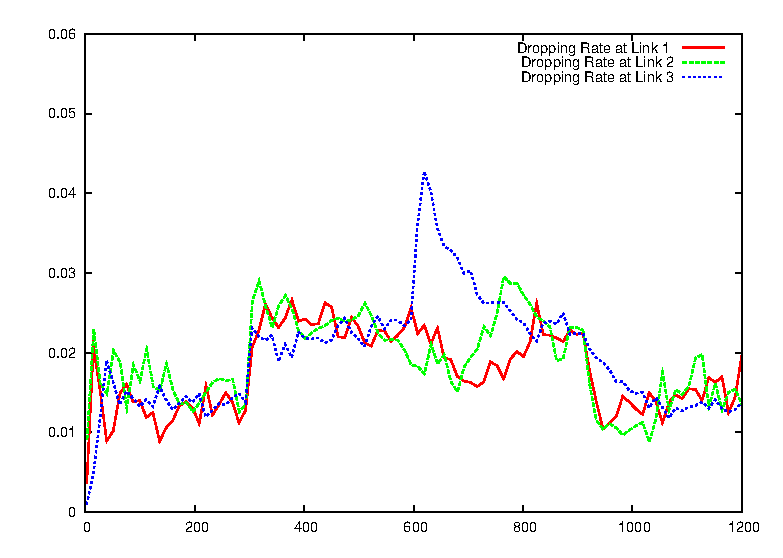
\epsfig{file=img/sec-5-2-1/eight/dropRate, width=4.5in}
\caption{
  Drop Rate at the botlenecks. 
    \label{fig:split-eight}
}
\end{center}
\end{figure}

%FLARE
 \begin{figure}[h!]
 \begin{center}
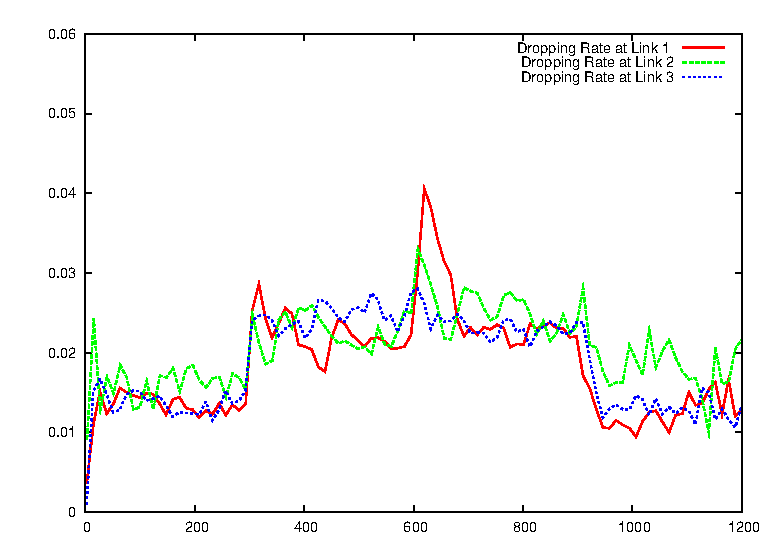
\epsfig{file=img/sec-5-2-1/four/dropRate, width=4.5in}
\caption{
  Drop Rate at the botlenecks.
    \label{fig:split-time-four}
}
\end{center}
\end{figure}

\clearpage

{\bf Update interval: 1sec}

\begin{figure}[h]
 \begin{center}

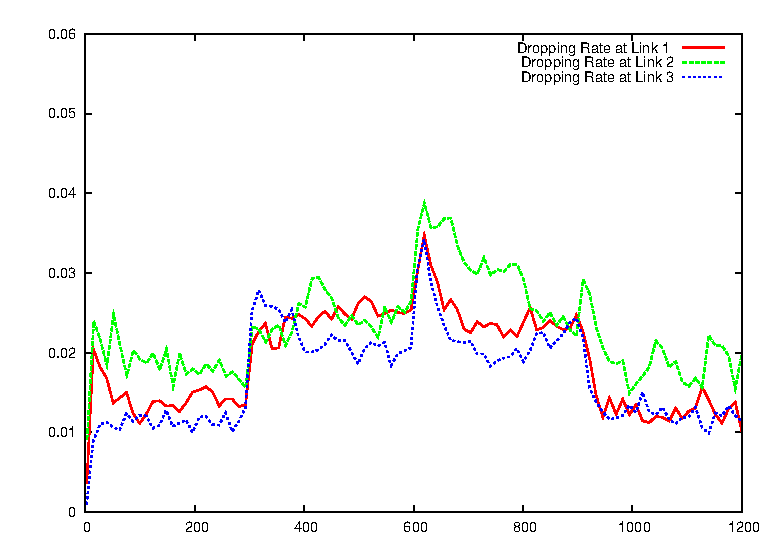
\epsfig{file=img/sec-5-2-1/one/dropRate, width=4.5in}
\caption{
  Drop Rate at the botlenecks.
    \label{fig:split-one}
}
\end{center}
\end{figure}

As expected, with a small update interval the algorithm acts more aggressively and doesn't leave enough time for the flows to reach stability. As a result the congestion level experienced in the different paths (expressed by the dropping rate at each bottleneck) is not well balanced. A larger time intervals (8 and 4 sec) allow to achieve a better balancing of the congestion over the available paths and with an enhanced stability. From the different simulations that we've carried out, an update interval between 40 to 100 RTT (approximately 100ms for the simulations here) allowed to achieve most of the time a good accuracy of the congestion balancing. An even higher value for the update interval turns the balancer too slow. This effect could be illustrated with the reaction of the system for sudden and important change in traffic demand. We could see at around the second 600, when the demand on traffic turned from a destination to another one, the balancer with an update interval of 4 sec required slightly less time to achieve equilibrium.    
 
 \clearpage

%\begin{figure}[htbp]
%\begin{center}
%\subfloat[]{
%\label{rcpstart4}
%\includegraphics[scale=0.4]{plots/lan/1.5Mb/rcp/flowstart4.eps}}
%\hspace{10mm}
%\subfloat[]{
%\label{xcprcpstart4}
%\includegraphics[scale=0.4]{plots/lan/1.5Mb/xcp0/flowstart4.eps}}
%\caption{The throughput of end-hosts and the router queue as a fourth flow starts, using \protect\subref{rcpstart4} RCP and \protect\subref{xcprcpstart4} XCP.}
%\label{rcpstart4comp}
%\end{center}
%\end{figure}

\subsection{PREFLEX balancing modes}

In this section we are going to analyse PREFLEX balancing mode: Equalization, Conservative and Loss Driven.

Reminder
$\beta_{E}$, $\beta_{C}$ and $\beta_{L}$ denotes positive factors associated consecutively with “equalization” $E$, “conservative” $C$, and “loss driven” $L$ modes.

{\bf Conservative mode} : $\beta_{E}=0$, $\beta_{C}=1$ and $\beta_{L}=0$
\\The conservative mode doesn't achieve an accurate congestion balancing over the available paths (figure \ref{fig:splitCon-loss}). But more importantly, the split as desired by the balancer in this mode is not stable(figure \ref{fig:splitCon-fwnd}). Thus, it can't be used to stabilize the performance of the balancer. A plausible explanation is limitation of the assumption that the flow fraction is equal to byte fraction, when the loss rates of paths aren't equivalent.

\begin{figure}[h!]
 \begin{center}

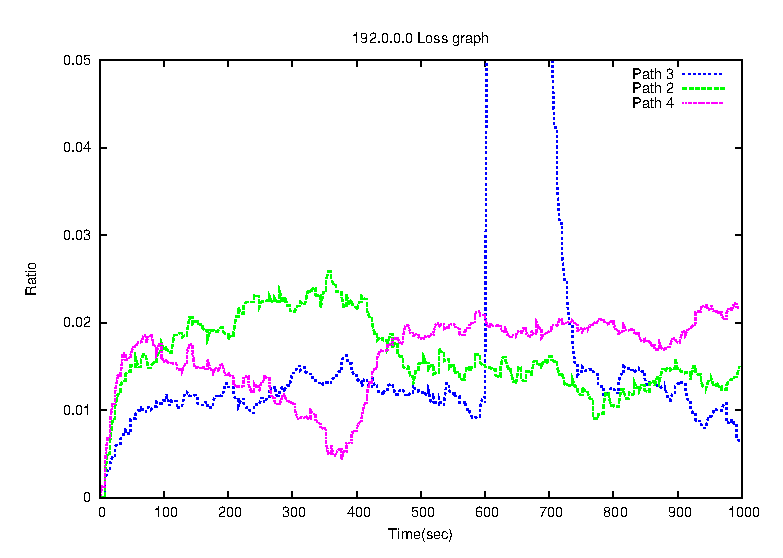
\epsfig{file=img/sec-5-2-2/Alt-split-0-100-0/loss-192-0-0-0, width=4.5in}
\caption{
   Loss ratio $\rho_{i}$ for destination E1 as seen by balancer P in consrvative mode.

    \label{fig:splitCon-loss}
}
\end{center}
\end{figure}

\clearpage
\begin{figure}[h!]
 \begin{center}

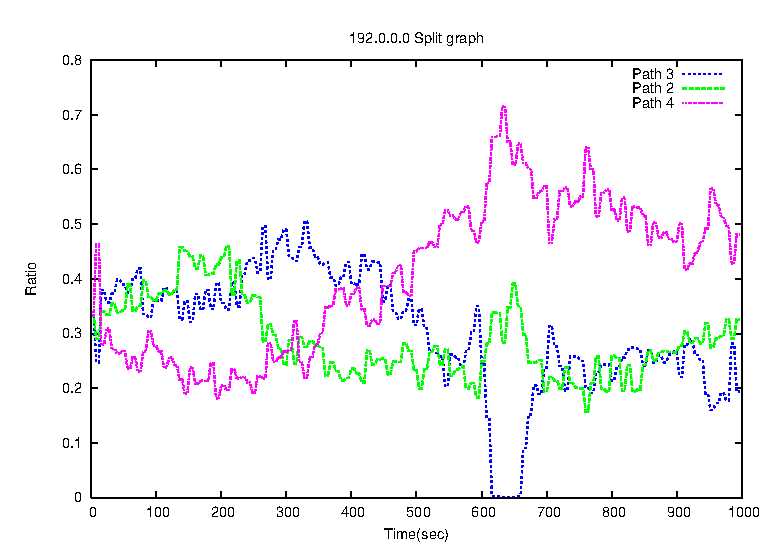
\epsfig{file=img/sec-5-2-2/Alt-split-0-100-0/fwnd-192-0-0-0, width=4.5in}
\caption{
   The desired split that balancer P set for destination E1 in conservative mode.

    \label{fig:splitCon-fwnd}
}
\end{center}
\end{figure}


{\bf Equalization} : $\beta_{E}=1$, $\beta_{C}=0$ and $\beta_{L}=0$
\\As depicted by figure \ref{fig:splitEqual-loss}, an equal distribution of flows over the paths doesn't achieve an equal balancing of loss. Moreover, its performance depends on the traffic nature in the network. Path 3 underutilized illustrates the suboptimal nature of equal balancing. Also the difference of congestion levels in the other two paths is directly linked to changes in traffic demand. During the change on traffic demand between time 200sec and 600sec, the difference between the congestion levels significantly increased.

However, the real contribution of the "equal" mode is to ensure that a minimum number of flows are sent over each path. In fact, as we are going to see next, the accuracy of the loss estimation made by the loss balancer depends on the number of flows sent over the path. 

\clearpage
\begin{figure}[h]
 \begin{center}

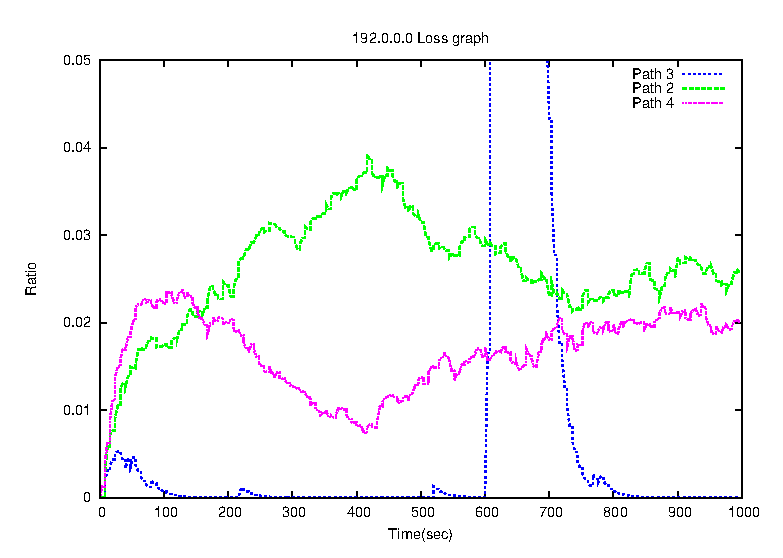
\epsfig{file=img/sec-5-2-2/Alt-split-0-0-100/loss-192-0-0-0, width=4.5in}
\caption{
   Loss ratio $\rho_{i}$ for destination E1 as seen by balancer P in equalisation mode.

    \label{fig:splitEqual-loss}
}
\end{center}
\end{figure}


{\bf Unbounded loss driven mode} : $\beta_{E}=0$, $\beta_{C}=0$ and $\beta_{L}=1$
\\Figures \ref{fig:splitpureLoss-fwnd1} and \ref{fig:splitpureLoss-fwnd1} show that the balancer allocate different splits for destination E1 and E2 even when the system is symmetric for the two destinations. This is explained by the fact that balancing for the two destination is carried separately which is natural since the flows for the two destinations. This is natural since the paths for the two destinations are different even if they share the same bottleneck in our topology. But there is no one optimal split, and the balancer succeeds though during the first 200 sec in balance the congestion equally for both destination (see \ref{fig:splitpureLoss-loss1} and \ref{fig:splitpureLoss-loss2}). But by keeping to send less E2 flows on the path, the accuracy of the loss estimation become low and different from E1 flows. In particular, it is over estimated what accelerate more the drop. As a result the equalization mode is used to make sure that there are enough flows on every path for an accurate estimation of the loss.

\begin{figure}[h]
 \begin{center}

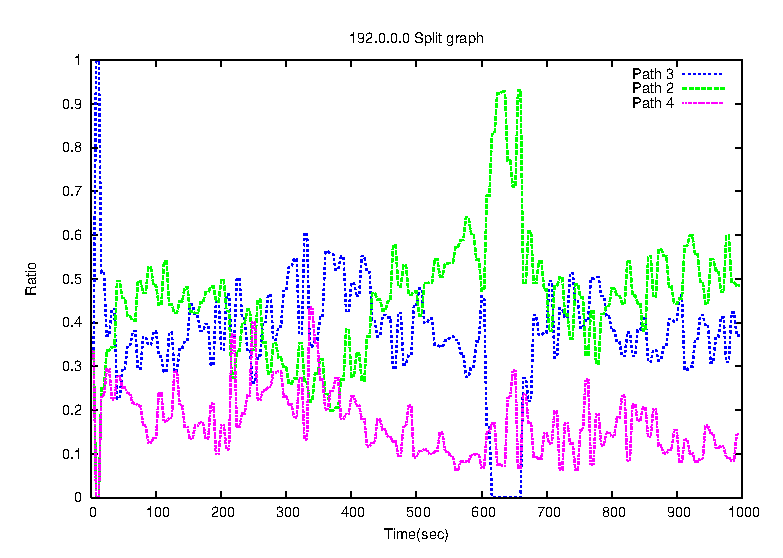
\epsfig{file=img/sec-5-2-2/Alt-split-100-0-0/fwnd-192-0-0-0, width=4.5in}
\caption{
   The desired split that balancer P set for destination E1 in unbounded loss driven mode.

    \label{fig:splitpureLoss-fwnd1}
}
\end{center}
\end{figure}

\begin{figure}[h]
 \begin{center}

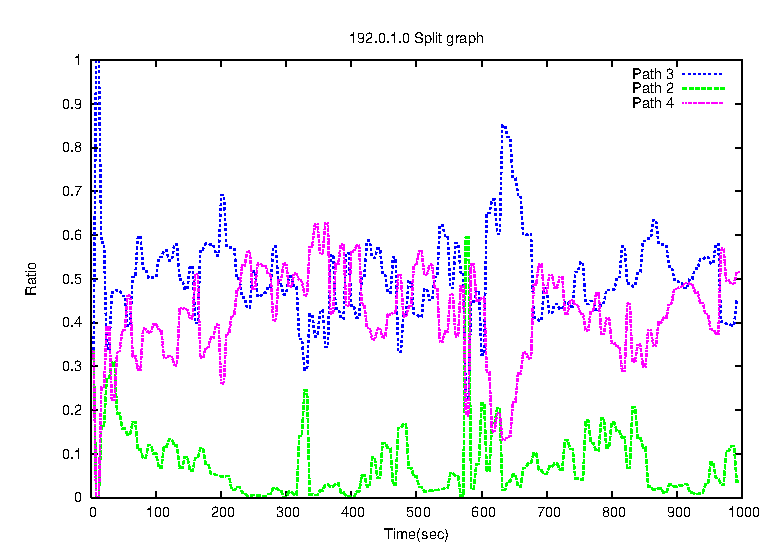
\epsfig{file=img/sec-5-2-2/Alt-split-100-0-0/fwnd-192-0-1-0, width=4.5in}
\caption{
   The desired split that balancer P set for destination E2 in unbounded loss driven mode.

    \label{fig:splitpureLoss-fwnd2}
}
\end{center}
\end{figure}


\begin{figure}[h]
 \begin{center}

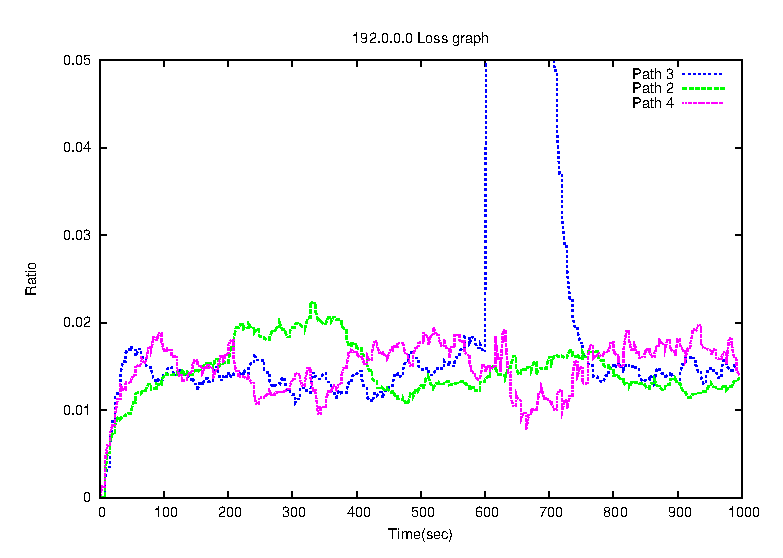
\epsfig{file=img/sec-5-2-2/Alt-split-100-0-0/loss-192-0-0-0, width=4.5in}
\caption{
   Loss ratio $\rho_{i}$ for destination E1 as seen by balancer P in unbounded loss driven mode.

    \label{fig:splitpureLoss-loss1}
}
\end{center}
\end{figure}

\begin{figure}[h]
 \begin{center}

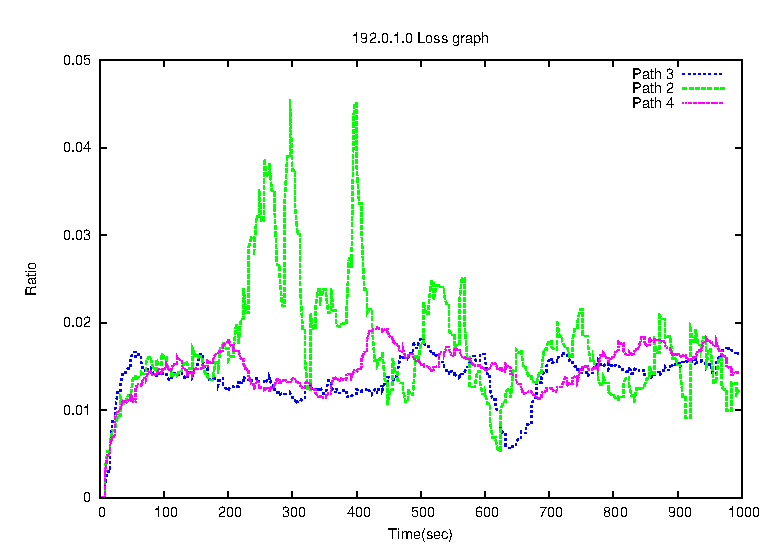
\epsfig{file=img/sec-5-2-2/Alt-split-100-0-0/loss-192-0-1-0, width=4.5in}
\caption{
   Loss ratio $\rho_{i}$ for destination E2 as seen by balancer P in unbounded loss driven mode.

    \label{fig:splitpureLoss-loss2}
}
\end{center}
\end{figure}

\clearpage

{\bf Bounded loss driven mode} : $\beta_{E}=0.9$, $\beta_{C}=0$ and $\beta_{L}=0.1$
\\By allocating a share of the traffic to be equally distributed we guarantee that a minimum number of flows is sent over each path to continue probing the path in question and accurately estimate its level of congestion. The effect of this boundary is clearly shown in the loss distribution compared to the previous mode \ref{fig:splitlossD-loss1} and \ref{fig:splitlossD-loss2}. Though, the  booked share for equalization should be too high to block the loss equalization process. 

In another hand, \ref{fig:splitlossD-fwnd1} and \ref{fig:splitlossD-fwnd1} {\bf Something about failure}


\begin{figure}[h]
 \begin{center}

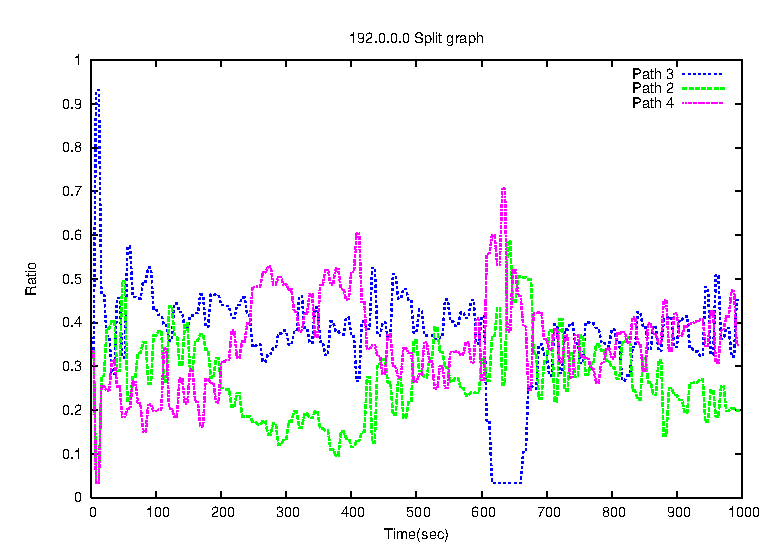
\epsfig{file=img/sec-5-2-2/Alt-split-90-0-10/fwnd-192-0-0-0, width=4.5in}
\caption{
   The desired split that balancer P set for destination E1 in "pure" loss driven mode.

    \label{fig:splitlossD-fwnd1}
}
\end{center}
\end{figure}

\begin{figure}[h]
 \begin{center}

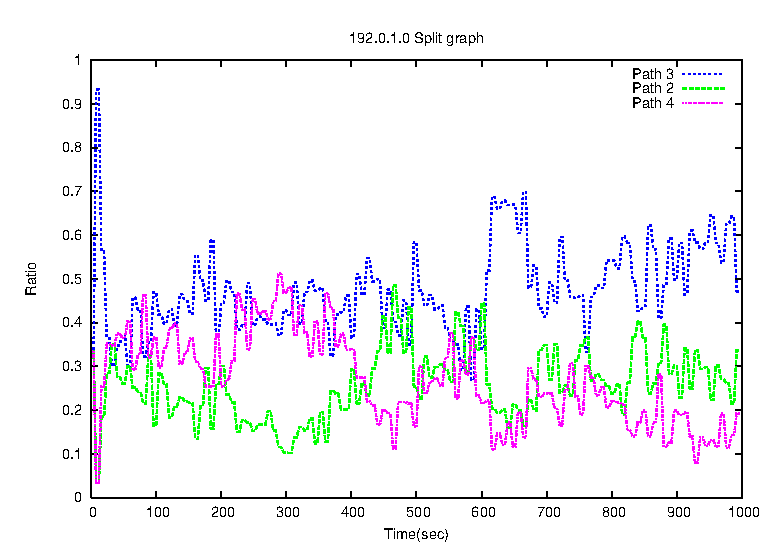
\epsfig{file=img/sec-5-2-2/Alt-split-90-0-10/fwnd-192-0-1-0, width=4.5in}
\caption{
   The desired split that balancer P set for destination E2 in "pure" loss driven mode.

    \label{fig:splitlossD-fwnd2}
}
\end{center}
\end{figure}


\begin{figure}[h]
 \begin{center}

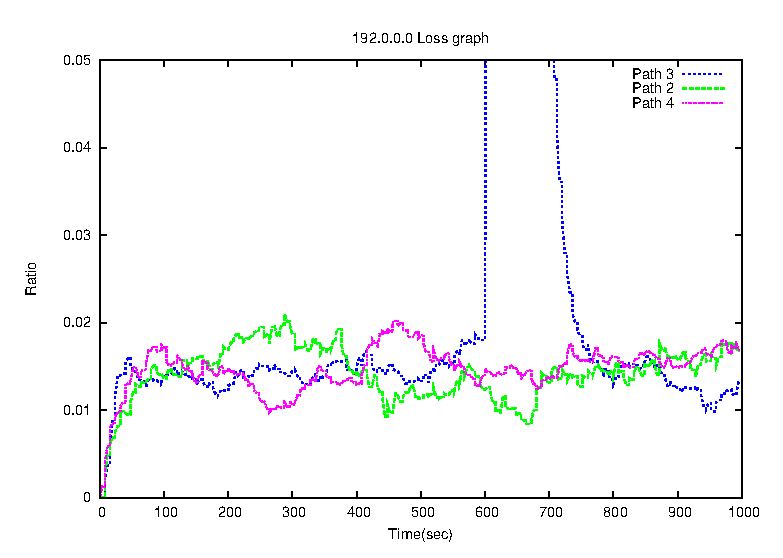
\epsfig{file=img/sec-5-2-2/Alt-split-90-0-10/loss-192-0-0-0, width=4.5in}
\caption{
   Loss ratio $\rho_{i}$ for destination E1 as seen by balancer P in "pure" loss driven mode.

    \label{fig:splitlossD-loss1}
}
\end{center}
\end{figure}

\begin{figure}[h]
 \begin{center}

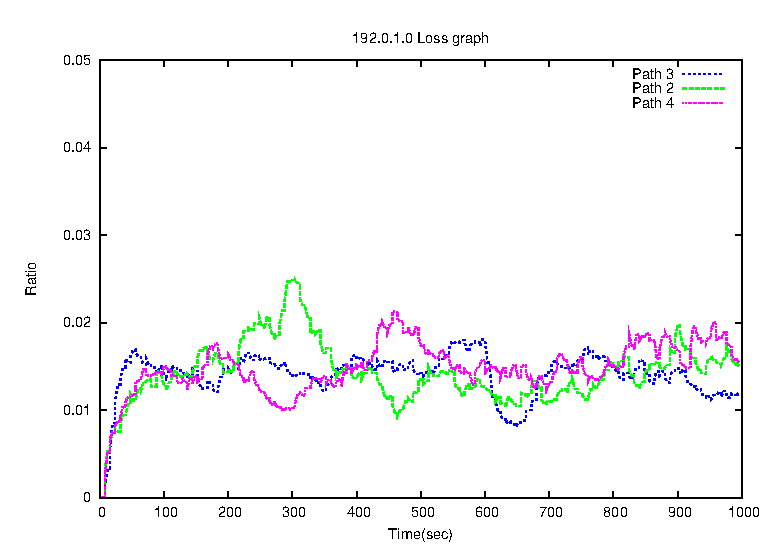
\epsfig{file=img/sec-5-2-2/Alt-split-90-0-10/loss-192-0-1-0, width=4.5in}
\caption{
   Loss ratio $\rho_{i}$ for destination E2 as seen by balancer P in "pure" loss driven mode.

    \label{fig:splitlossD-loss2}
}
\end{center}
\end{figure}

\clearpage

\section{Comparison between PREFLEX and TEXCP}

{\bf Balancing by path utilization}
\\In this section we consider a simplified version of TEXCP (the same as in 5.1.1) that balances path utilization but doesn't activate TEXCP congestion management measures and only balance the path utilization. As expected (figure \ref{fig:st-util}), the modified version do very well in equalizing the path utilization, reacting very quickly to changes in network traffic state while keeping a stable behavior. 

However, by looking at the drop rate in bottlenecks (figure \ref{fig:st-drop}) we observe that it is not equal on the different links. This observation, have a meaningful explanation behind. The high frop rate on the likn is compensated by a higher load (received bytes over the capacity) so the utilization is equal on the three links. This means that using only this measure for balancing the load we risk to drive the network to a suboptimal state. The other observation is about the loss level that ingress routers see using LEX codepoint (figure \ref{fig:st-loss1}). All the three interfaces, which correspond to the links, have the same level. This is an expected results since TEXP use FLARE which doesn't guarantee that retransmissions follow the same path as the original packet. This have another result is that within dew RTTs, TCP routines using different paths experience the congestion of each of them and hence they adapt their transmission rate to a combination of loss rate in each path that could be estimated as:

\begin{equation}
\rho = \sum_{i} x_{i}\cdot \rho_{i} 
\end{equation}

where, $\rho_{i}$ and $x_{i}$ are respectively the loss rate and the probability to take path i. But we should keep in mind that such high levels of path utilization aren't frequent in intra-domain TE, since not all the flows are elastic as it is the case in our scenario. For such cases, TEXCP defines a feedback mechanism to control congestion.

\begin{figure}[h]
 \begin{center}

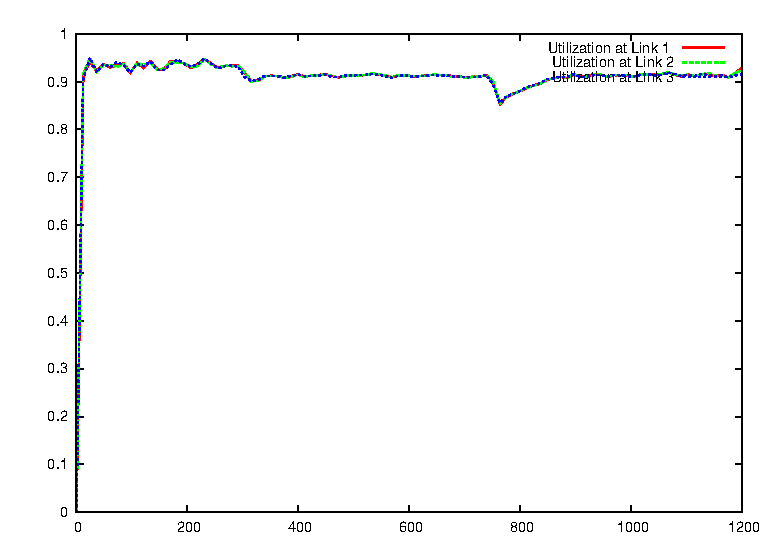
\epsfig{file=img/sec-5-2-3/no-traffic-shaper/util, width=4.5in}
\caption{
   The link utilization measured at the bollenecks in simplified TEXCP.

    \label{fig:st-util}
}
\end{center}
\end{figure}

\begin{figure}[h]
 \begin{center}

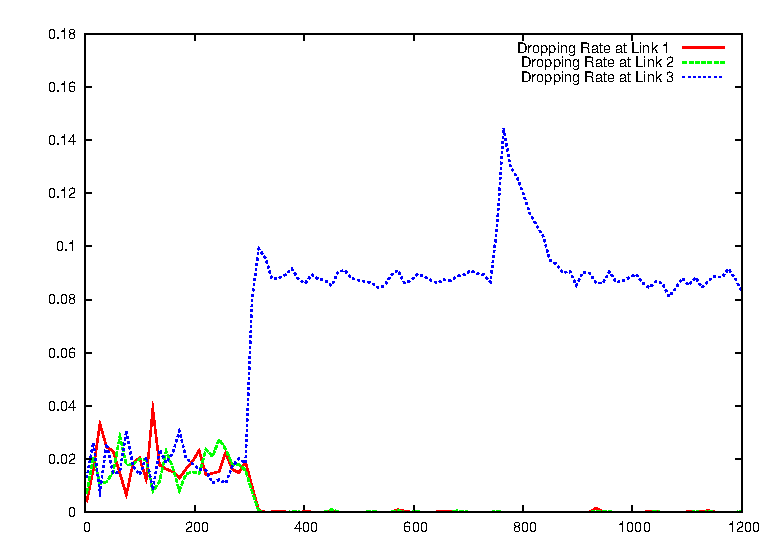
\epsfig{file=img/sec-5-2-3/no-traffic-shaper/dropRate, width=4.5in}
\caption{
   The drop rate measured at the bollenecks in simplified TEXCP.

    \label{fig:st-drop}
}
\end{center}
\end{figure}

\begin{figure}[h]
 \begin{center}

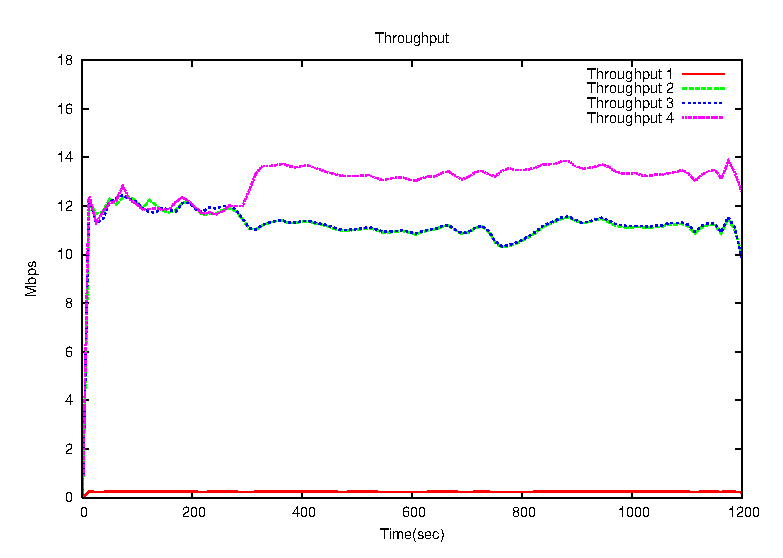
\epsfig{file=img/sec-5-2-3/no-traffic-shaper/10/throuputs, width=4.5in}
\caption{
   The throughput measured at ingress router I1 interfaces in simplified TEXCP.

    \label{fig:st-fwnd}
}
\end{center}
\end{figure}

\begin{figure}[h]
 \begin{center}

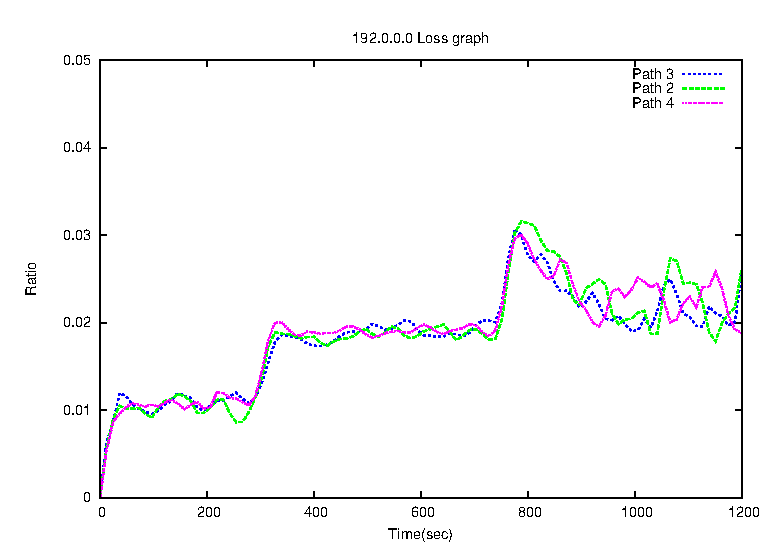
\epsfig{file=img/sec-5-2-3/no-traffic-shaper/10/loss-192-0-0-0, width=4.5in}
\caption{
   Loss ratio $\rho_{i}$ for destination E1 as seen by balancer ingress router I1 in simplified TEXCP.

    \label{fig:st-loss1}
}
\end{center}
\end{figure}
\clearpage 

{\bf TEXCP}

\\In this section TEXCP was fully implemented. A traffic shaper is associated with each Ingress/Egress route and control the transmission rate over the different paths. The path utilization is still equalized for the three bottlenecks (figure \ref{fig:t-util}), but most importantly the difference in drop rate ???? at each link disappeard (\ref{fig:t-drop}). The path utilization has slightly increase, which is correlated with the decrease in the drop rate at the bottleneck since TCP routing under low loss rate have a stable transmission rate and doesn't fluctuate a lot. By limiting the transmission rate, the effect of the traffic shaper is to move congestion and more precisely the dropping from the core network to the edge. 

The introduction of traffic shapers changes the loss rate. Indeed, traffic shaper allocates a buffer for each destination instead of the common buffer at the bottlneck. In our topology each link pass through the traffic of four IE pairs. Using traffic shapers means that four queues will be added. The number of added queue and their size are new parameters to influence the level of congestion. For instance the ratio buffer size over the transmission rate could decrease significantly the global loss rate if set to a high value, and the inverse is true. The mathematical formalization of this problem is quite difficult.

But the drawback of the use traffic shapping and transmission rate control, is to equally distributed bandwidth over pairs but not according to the size of traffic travelling between them. In general this results in a bandwidth waste since some of the users won't be able to use all their share. But since we are using elastic flow the bandwidth is fully used, yet the level of loss is different from a destination to another (figure \ref{fig:t-loss1} and \ref{fig:t-loss2}). Starting from the moment when the bottlenecks feel congested, the transmission rate of each pair and path is decreased. The decrease mechanism is multiplicative, so if the transmission rates were defined equally at the beginning they will reach the same equilibrium. This is fine while they have equal number of flows but once this distribution change the different flows will keep having equal rates. This means that the level of congestion experience for one destination is different from another even if they share the same bottleneck. Hence the use of traffic shappers introduce unfairness.

\begin{figure}[h]
 \begin{center}

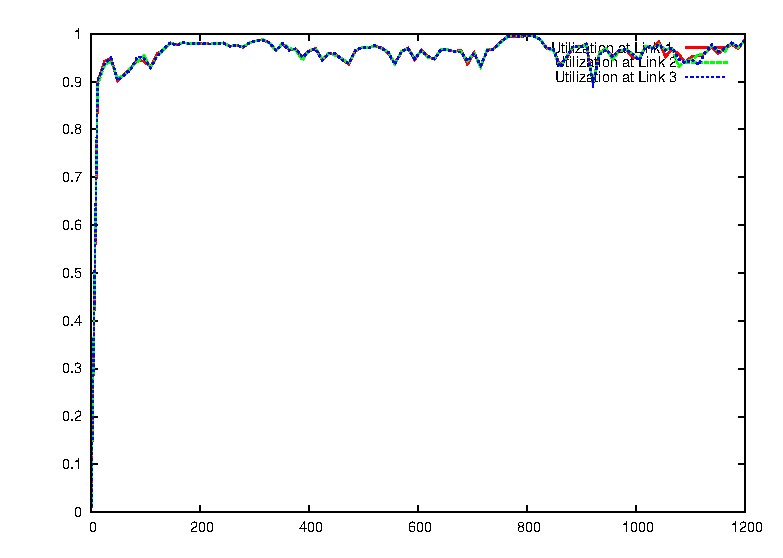
\epsfig{file=img/sec-5-2-3/trafficShaper/util, width=4.5in}
\caption{
   The link utilization measured at the bollenecks in TEXCP.

    \label{fig:t-util}
}
\end{center}
\end{figure}

\begin{figure}[h]
 \begin{center}

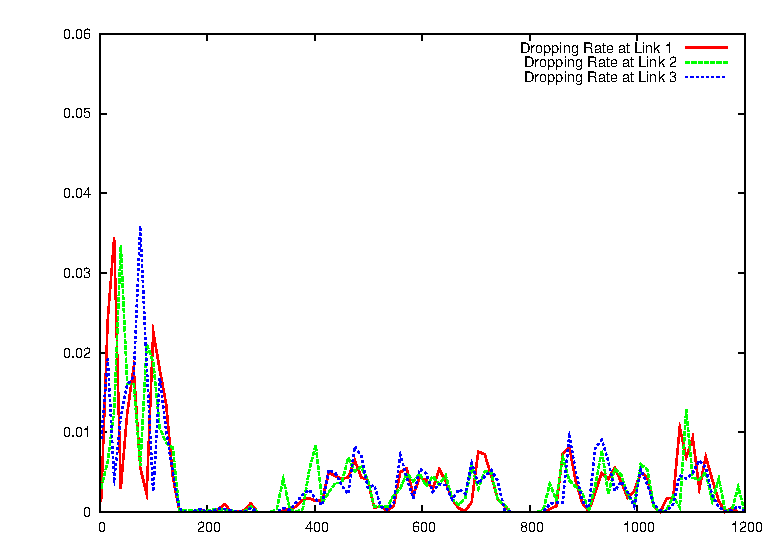
\epsfig{file=img/sec-5-2-3/trafficShaper/dropRate, width=4.5in}
\caption{
   The drop rate measured at the bollenecks in TEXCP.

    \label{fig:t-drop}
}
\end{center}
\end{figure}

\begin{figure}[h]
 \begin{center}

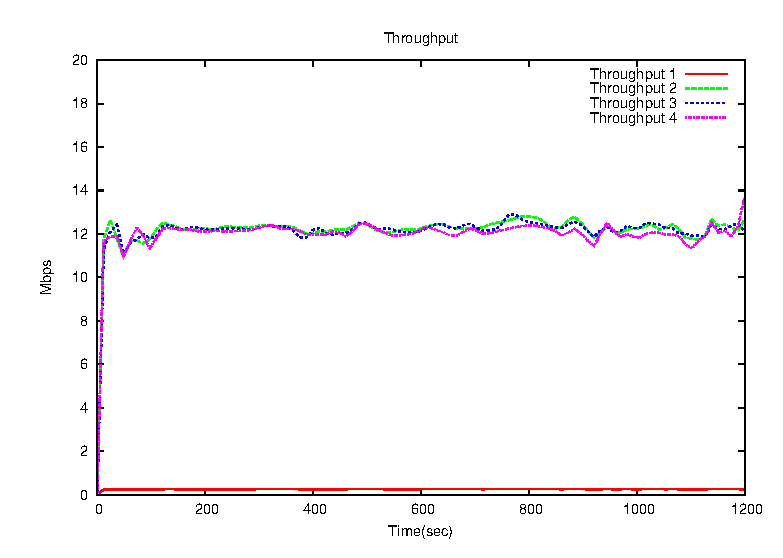
\epsfig{file=img/sec-5-2-3/trafficShaper/10/throuputs, width=4.5in}
\caption{
   The throughput measured at ingress router I1 interfaces in TEXCP.

    \label{fig:t-fwnd}
}
\end{center}
\end{figure}

\begin{figure}[h]
 \begin{center}

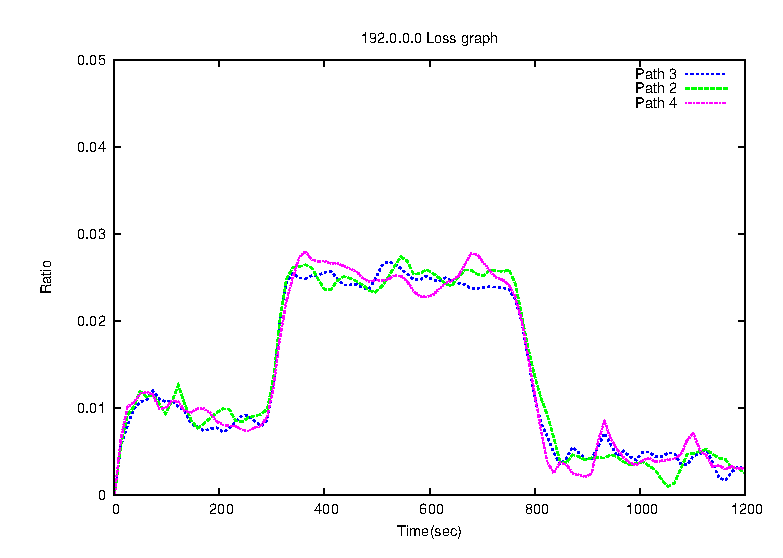
\epsfig{file=img/sec-5-2-3/trafficShaper/10/loss-192-0-0-0, width=4.5in}
\caption{
   Loss ratio $\rho_{i}$ for destination E1 as seen by balancer ingress router I1 in TEXCP.

    \label{fig:t-loss1}
}
\end{center}
\end{figure}

\begin{figure}[h]
 \begin{center}

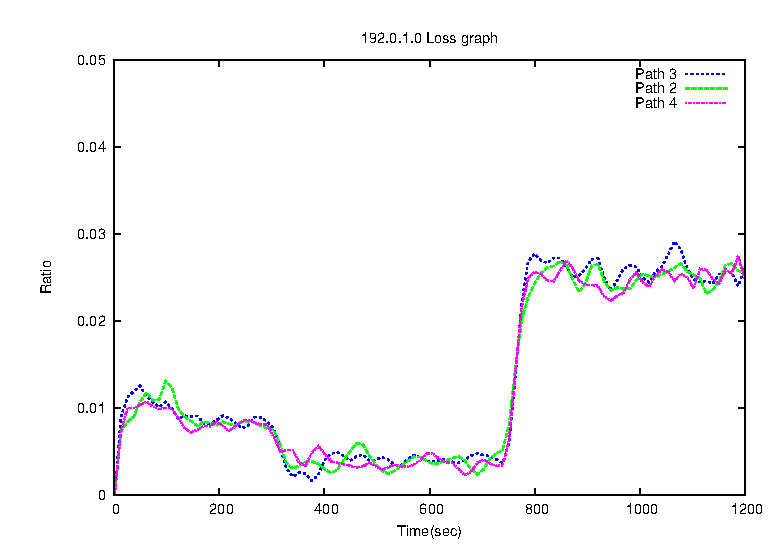
\epsfig{file=img/sec-5-2-3/trafficShaper/10/loss-192-0-1-0, width=4.5in}
\caption{
   Loss ratio $\rho_{i}$ for destination E2 as seen by balancer ingress router I1 in TEXCP.

    \label{fig:t-loss2}
}
\end{center}
\end{figure}

\clearpage 

{\bf PREFLEX}
\\ In this section a comparison is carried out with congestion balancing in PREFLEX. The congestion parameters of the balancing algorithm were set to : $\beta_{E}=0.9$, $\beta_{C}=0$ and $\beta_{L}=0.1$.

PREFLEX performance in balancing congestion is similar to the one obtained in the previous section for the same configuration (Analysis of PREFLEX balancing algorithm 5.2.2). 


\begin{figure}[h]
 \begin{center}

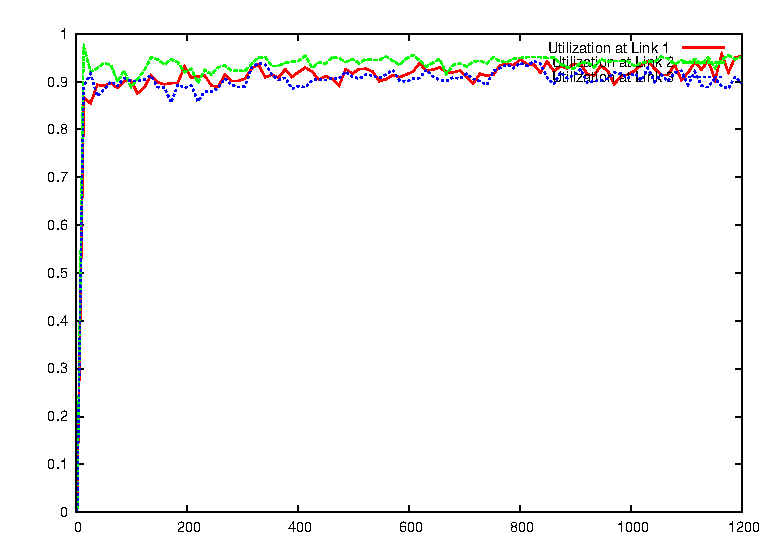
\epsfig{file=img/sec-5-2-3/split-90-0-10/util, width=4.5in}
\caption{
   The link utilization measured at the bollenecks in TEXCP.

    \label{fig:p-util}
}
\end{center}
\end{figure}

\begin{figure}[h]
 \begin{center}

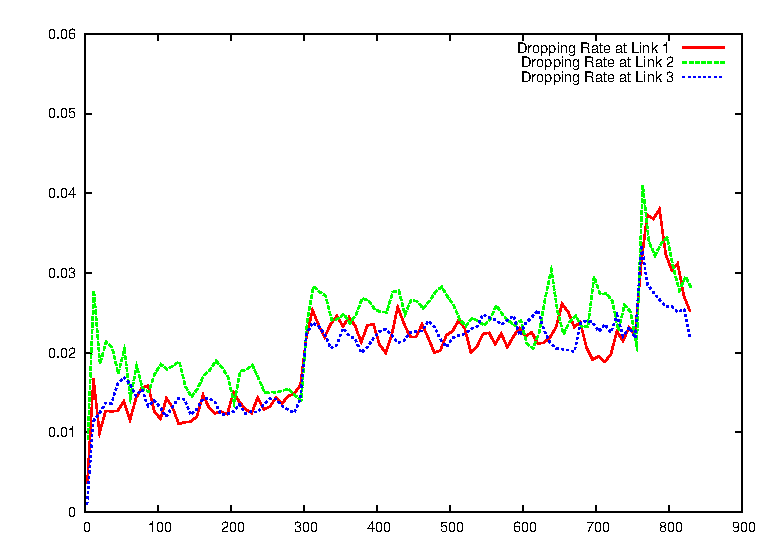
\epsfig{file=img/sec-5-2-3/split-90-0-10/dropRate, width=4.5in}
\caption{
   The drop rate measured at the bollenecks in TEXCP.

    \label{fig:p-drop}
}
\end{center}
\end{figure}

\begin{figure}[h]
 \begin{center}

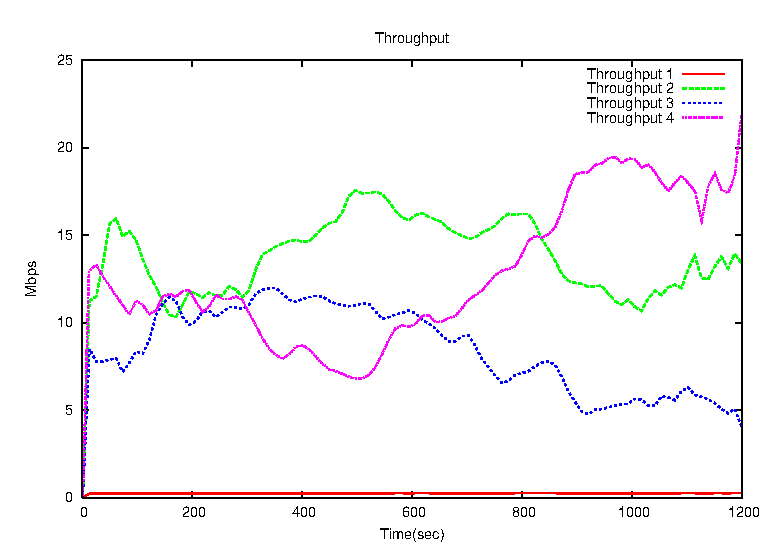
\epsfig{file=img/sec-5-2-3/split-90-0-10/10/throuputs, width=4.5in}
\caption{
   The throughput measured at ingress router I1 interfaces in TEXCP.

    \label{fig:p-fwnd}
}
\end{center}
\end{figure}

\begin{figure}[h]
 \begin{center}

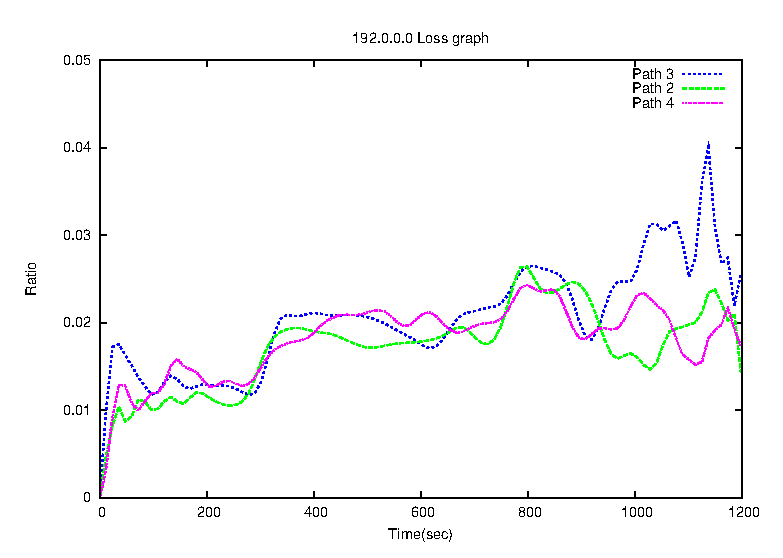
\epsfig{file=img/sec-5-2-3/split-90-0-10/10/loss-192-0-0-0, width=4.5in}
\caption{
   Loss ratio $\rho_{i}$ for destination E1 as seen by balancer ingress router I1 in TEXCP.

    \label{fig:p-loss1}
}
\end{center}
\end{figure}

\begin{figure}[h]
 \begin{center}

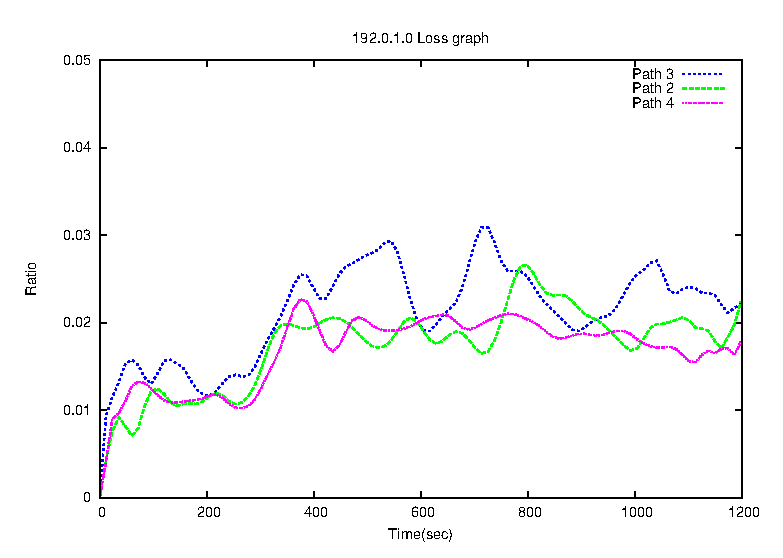
\epsfig{file=img/sec-5-2-3/split-90-0-10/10/loss-192-0-1-0, width=4.5in}
\caption{
   Loss ratio $\rho_{i}$ for destination E2 as seen by balancer ingress router I1 in PREFLEX.

    \label{fig:p-loss2}
}
\end{center}
\end{figure}
